\chapter{Project Management}
\label{ch:project-management}
% https://warwick.ac.uk/fac/sci/dcs/teaching/material/cs310/components/final/marking/management
% https://warwick.ac.uk/fac/sci/dcs/teaching/material/cs310/reusingcontent

\section{Specification}
\label{sec:specification}
% Did the student make clear at the start of the project what they intended to do?

At the start of the project, a set of MoSCoW prioritised \cite{CaseMethodFastTrack} requirements was created, which fully defined concrete goals for the project. These are included in Appendix \ref{sec:project-requirements}. These fixed requirements gave the project a clear overall goal from a very early stage, and helped adopt good planning and development methodologies. These methodologies are discussed in the next section, \ref{sec:organisation}.

\section{Organisation}
\label{sec:organisation}
% Did the student plan their activities in advance and keep to the plan? Did the student exhibit good time-management skills?

\subsection{Project plan}
\label{ssec:organisation-plan}
% Gantt chart and planning

\subsection{Development methodology}
\label{ssec:organisation-methodology}

% What is an Agile methodology


\begin{figure}[h]
    \centering
    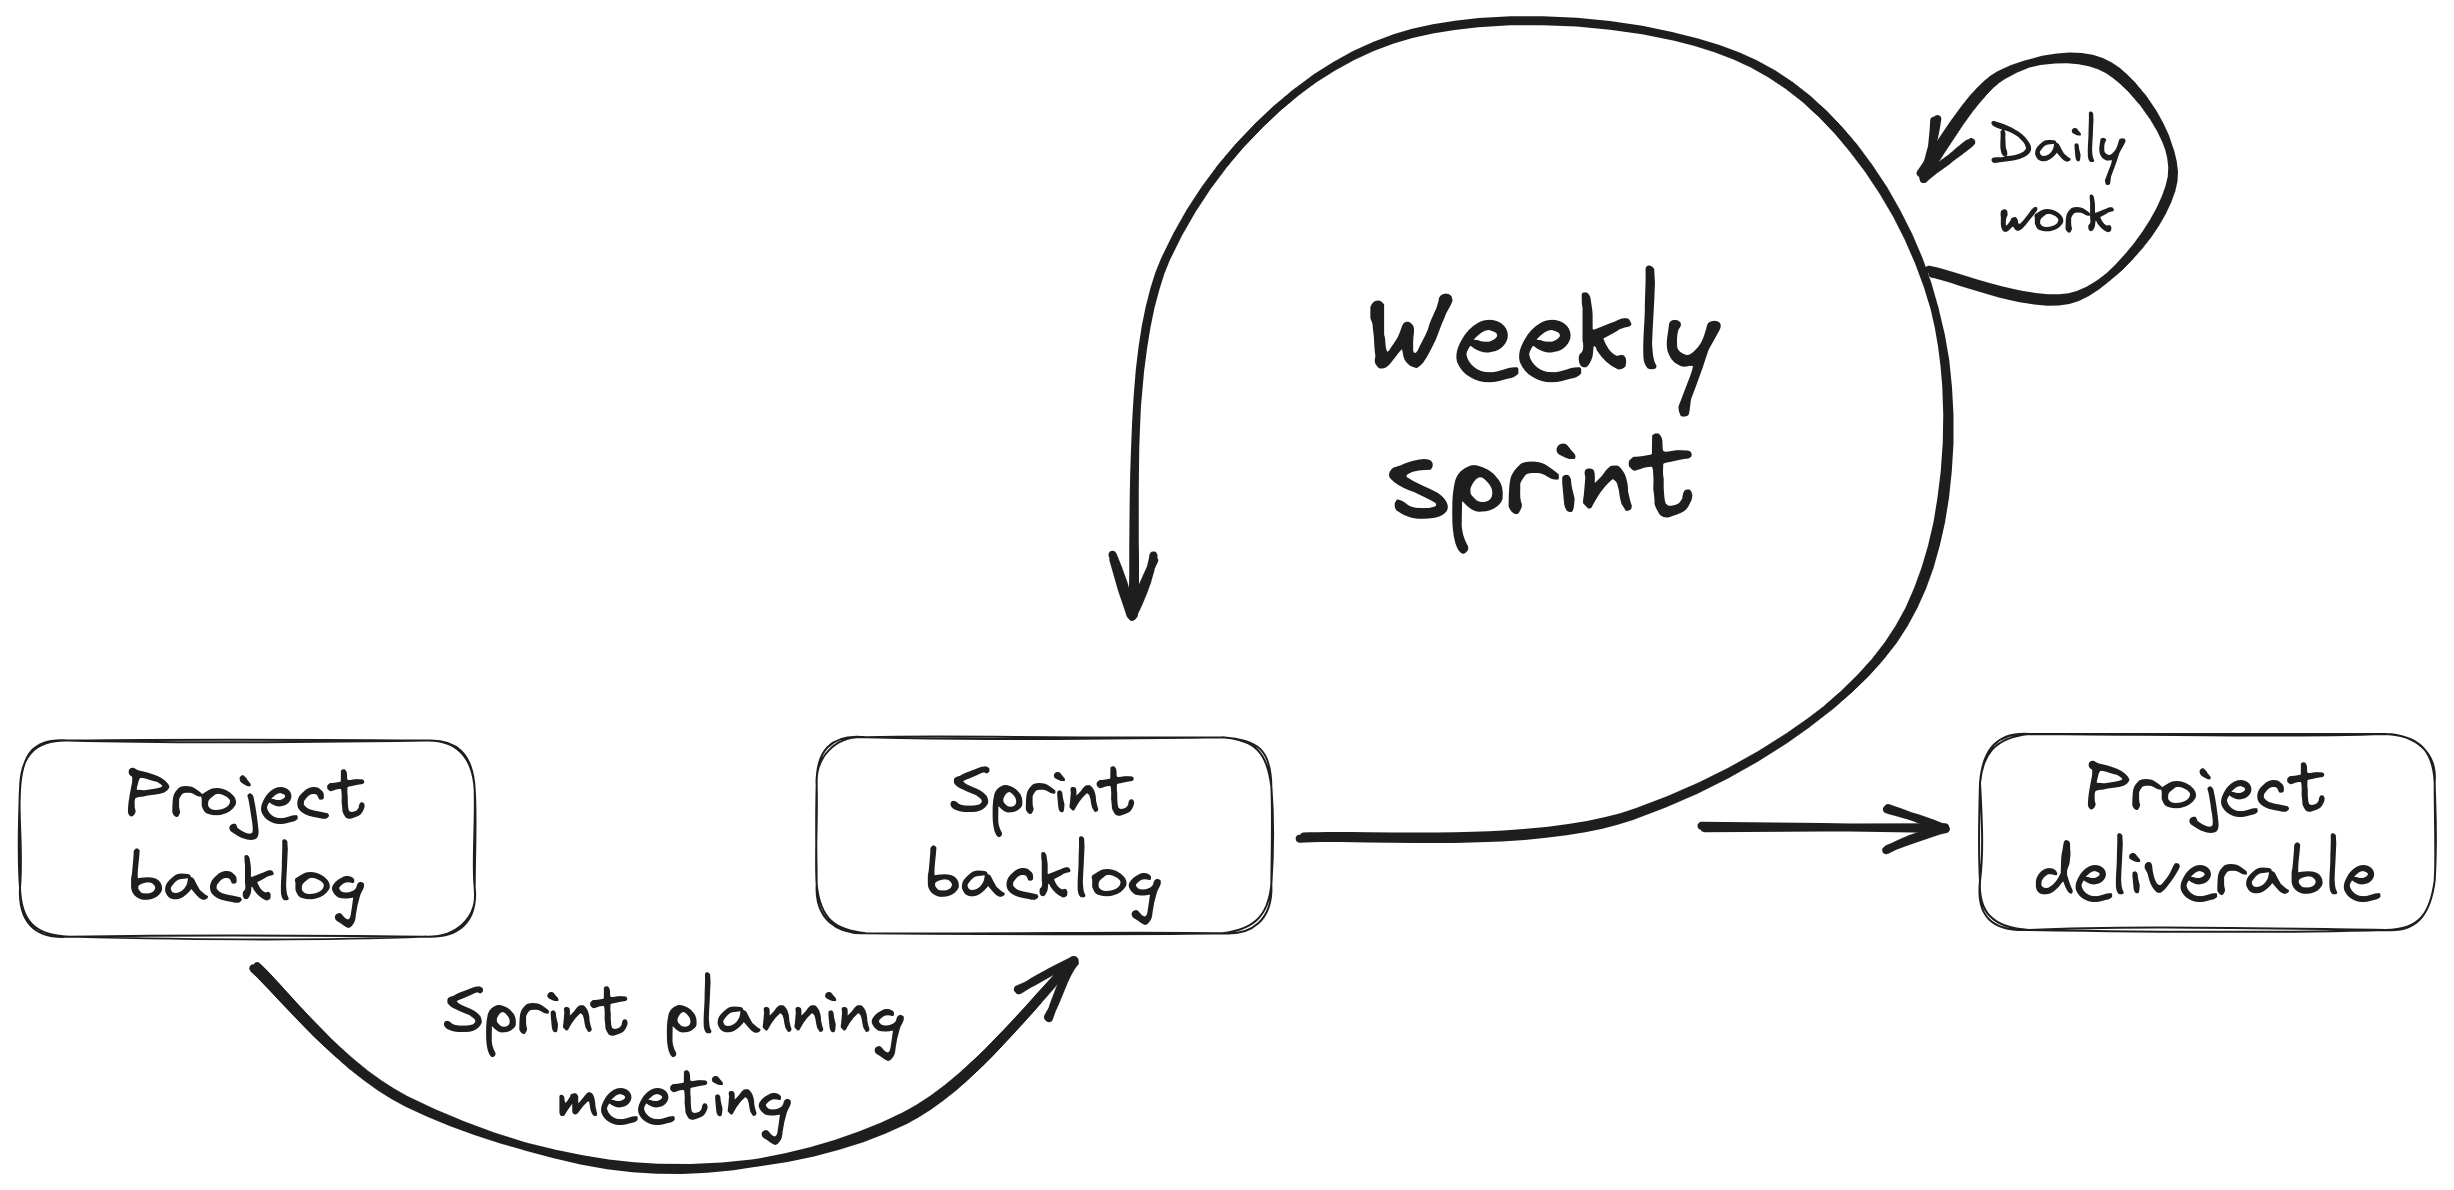
\includegraphics[width=0.75\textwidth]{images/6_project_management/excalidraw_agile.png}
    \caption{A diagram of a typical workflow for the Scrum flavour of Agile development.}
    \label{fig:excalidraw_agile}
\end{figure}

% Tools selected for use

\subsection{Responding to unforeseen issues}
\label{ssec:organisation-unforeseen-issues}

As discussed in the previous section, \ref{ssec:organisation-methodology}, following an Agile methodology empowered the project to be flexible to change, allowing the original plan to be adapted based on new information or ongoing supervisor discussions. A concrete example of this is the development of the HPC MultiBench tool was not an explicit project requirement enumerated in the specification, but following identification of a need and supervisor discussion, it was included as part of the performance analysis requirements. This successful deviation from the initial project plan also supports the fact that the chosen methodology would have been robust against major unforeseen issues, had any occurred.

% TODO: typeset risk matrix better, or move to appendix
In the project specification, a Risk Matrix characterising possible issues was generated, as shown in Table \ref{tab:risk_matrix}.
Of these identified possible risks, the only one which manifested itself was compute resources becoming busy, which is consistent with it having the highest estimated likelihood. This had a low impact on the project progress, as I had access two resources (both \texttt{kudu} on DCS and \texttt{Avon} on SCRTP), and could switch to other tasks whilst waiting for long jobs to complete.


% When generating the Risk Matrix for the specification, some possible risks were excluded, such as personal computer failure. However, this was experienced multiple times during the project

\begin{table}[H]
\begin{adjustwidth}{-3em}{-3em}
    \centering
    \caption{The proposed Risk Matrix for the project, from the project specification.}
    \label{tab:risk_matrix}
    \begin{tabular}{|p{0.2\linewidth}|p{0.25\linewidth}|p{0.065\linewidth}|p{0.085\linewidth}|p{0.055\linewidth}|p{0.24\linewidth}|} \hline
         Risk&  Cause of risk&  Bad- ness&  Likeli- hood&  Score& Mitigation strategy\\ \hline
         Major upheaval of the Rust language&  The Rust Foundation making a controversial decision \cite{AmNoLonger2023} \cite{AddRFCGovernance} \cite{TelemetryGoToolchain}&  4&  1&  \cellcolor{green!25}4 & Use a previous edition of Rust via \texttt{rustup}\\ \hline 
         Data structure for selected mini-app cannot be recreated under Rust's memory safety
  constraints&  Some data structures cannot be represented with Rust's ownership model, such as doubly linked lists \cite{leeBuildingMemorysafeNetwork2017}&  5&  6&  \cellcolor{red!25}30& Create a safe API around the required unsafe data structure\\ \hline 
         Compute resources become busy slowing development and testing&    In late term two many students use \texttt{kudu} for courseworks and dissertations&  2&  8&  \cellcolor{orange!25}16& Use a different compute resource, for example if \texttt{kudu} is busy use SCRTP or local machines\\ \hline 
         Unable to install Rust on compute resources&  Some compute resources may have restrictive permissions for users&  9&  3&  \cellcolor{red!25}27& Install only for a single user, or leverage containerisation to avoid installation issues\\ \hline 
 Loss of access to IBM computer resources or mentor and connections& Internal changes to IBM unrelated to the project& 4& 1& \cellcolor{green!25}4 &Whilst the IBM resources are nice to have, none of them are essential to the project, so can just continue without them\\ \hline
    \end{tabular}
    \end{adjustwidth}
\end{table}

\section{Effort and motivation}
\label{sec:effort-and-motivation}
% Did the student work hard?

I believe this project could be described as high effort through deeply consistent work. In the first term, I had no timetabled activities on Fridays, so set them aside as a time to work exclusively on the project, without incurring the cost of context switching to other activities. This allowed me to make strong progress, completing the translation and parallelisation objectives ahead of schedule. In the new year, I came up with and undertook a challenge along with a group of friends to make a project-related \texttt{git} commit every day during the month of January (``proj-anuary'', a portmanteau of project and January). I then chose to continue this for the entirety of the second term of this academic year, as shown in Figure \ref{fig:github_year_long_contributions}.

\begin{figure}[h]
    \centering
    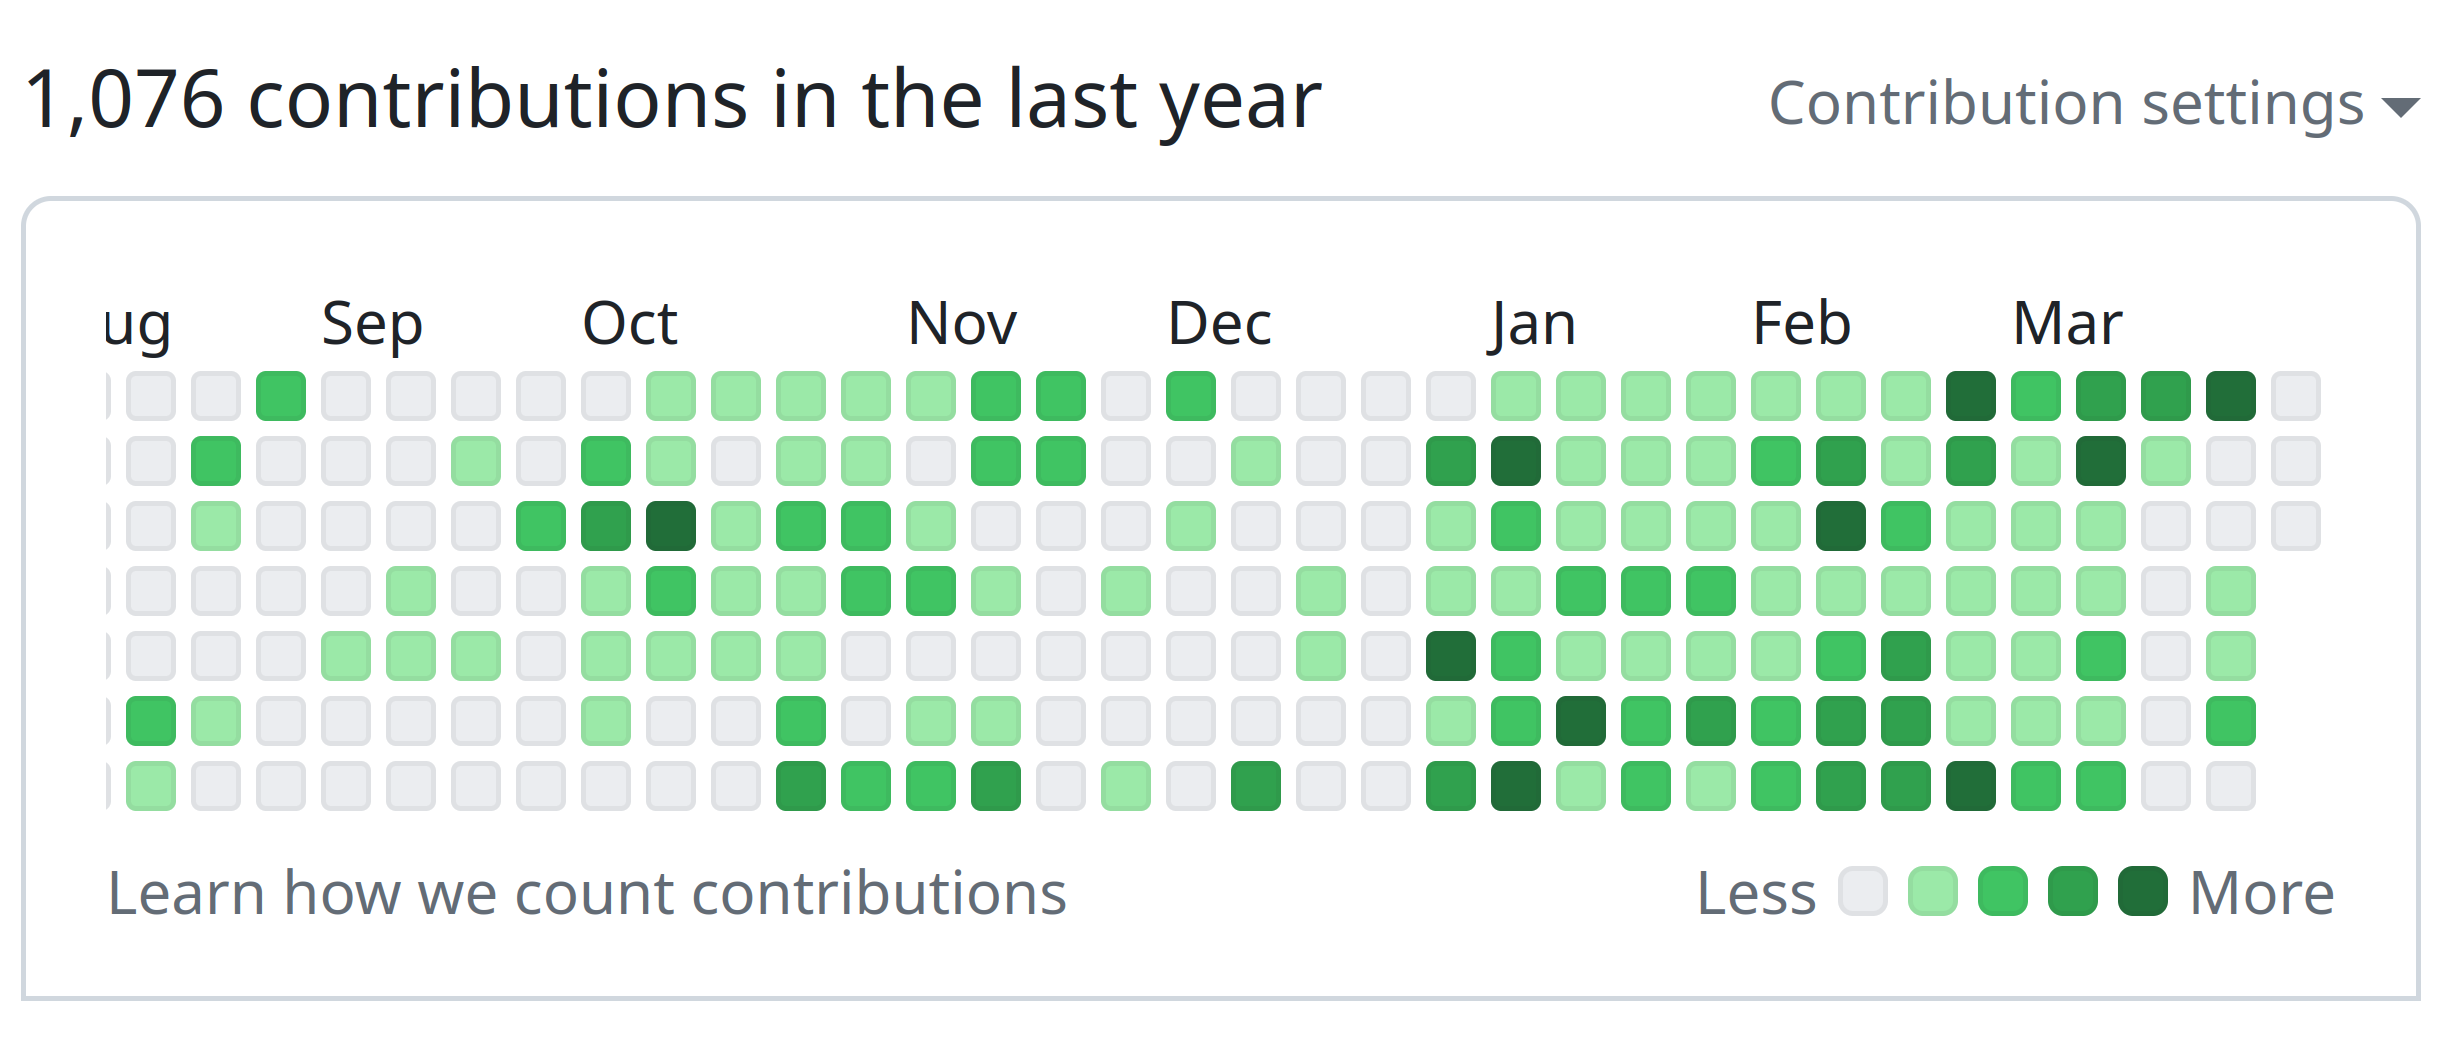
\includegraphics[width=0.75\textwidth]{images/6_project_management/github_year_long_contributions.png}
    \caption{A diagram showing my GitHub contributions over the past academic year. Commits from January 1\textsuperscript{st} to March 18\textsuperscript{th} form an unbroken consecutive streak of 78 days.}
    \label{fig:github_year_long_contributions}
\end{figure}

This punctilious approach to project progression paid great dividends, with even stronger progress being made in the second term than the first. This included successfully completing the stretch goal of running Rust code across clustered compute resources using MPI, and building the HPC MultiBench tool for generalised performance analysis of software executed via Slurm.

\section{Legal, social, ethical, and professional issues}
\label{sec:legal-social-ethical-professional-issues}
% Has the student taken into account matters such as ethics, social issues, and the law, as they relate to the project?

At the start of the project, any possible legal, social, ethical, and professional issues relating to the project were identified. 

Firstly, a small number of legal issues could relate the the project, largely relating to software licensing. Since High-Performance Computing is an active field of development in industry, some libraries or tools may have restrictive licences, so care was taken when picking and using tools to conform to the terms of their licences. Additionally, when identifying possible legal issues in the specifcation, it was noted that some mini-applications in the Mantevo suite are based on simulations of experiments in nuclear physics, so working with them might require special care to conform to relevant UK law. However, this issue was mitigated by selecting to examine the HPCCG mini-application \cite{herouxHPCCGSolverPackage2007}, which is instead based on methods of conjugate gradients solving linear systems \cite{hestenesMethodsConjugateGradients1952}.

Secondly, a level of professionalism is required for all projects. This project does not necessitate any professional considerations above basic norms, such as making meaningful commit messages, or avoiding profanity in source code comments. % TODO: Change this list of basic norms

Finally, since this project does not use human-generated data (for example data from surveys), nor is it creating a product humans directly use, it does not have any notable ethical nor social considerations. This was verified by following the flowchart on the \href{https://warwick.ac.uk/fac/sci/dcs/teaching/ethics}{ethical consent page of the project website}. % TODO: Could argue that shift to building HPC multibench requires social considerations

Due to the importance of these categories of issues, they were reviewed again for any changes at the midpoint of the project when writing the progress report, and yet again at the end when writing the final report. Since the project remained broadly fixed in scope, no additional issues were identified at these points.

In summary, this project carefully considered all relevant legal, social, ethical, and professional issues pertaining to the project, 

